\documentclass[12pt, letterpaper]{article}
\usepackage[utf8]{inputenc}
\usepackage{graphicx}
\usepackage{hyperref}
\usepackage{fancyvrb}
\usepackage{array}


\title{Rapport de projet : Bibliothèque génerale au developpement de jeux de Carte}
\author{Vincent Auconie \& Chaolei CAI
\\ 
  \multicolumn{1}{
      p{.7\textwidth}}{\centering\emph{Université de Paris \\
  UFR Informatique\\}
  M1 Informatique}
}

\date{\today}

\begin{document}


\begin{titlepage}
    \maketitle
\end{titlepage}

\tableofcontents

\section{Avant propos}
Notre projet est donc de développer un framework générale qui permet de géneraliser certaines tâches lors 
du developpement d'un jeu de carte. \\
Un README.ME est incluse dans le fichier, il contient quelques explications quand à l'utilisation et compilation de la bibliothèque ainsi que les jeux que 
nous avons développés.\\
Il existe un dépôt github si jamais vous avez un souci avec le dossier .zip ou .rar\\
\url{https://github.com/bk211/Projet-POO-M1}

\subsection{Compatibilité et environnement}
La bibliothèque ainsi que les jeux ont été développé en intégralité sous le standard c++11, avec le compilateur g++.
Il est livré sans warning, sans bug(enfin j'espère).\\ 
Niveau compatibilité, cela ne devrait pas poser de problème que vous soyez sous Linux ou windows.\\
Sur la plateforme Windows, l'usage de PowerShell est déconseillé car certaines commandes make ne sont pas exécutable depuis ce shell. 
Utilisez plutôt un shell type git-bash ou cgywin.


\section{Présentation de la bibliothèque}
Le premier point important qui caractérise notre bibliothèque est qu'il est polymorphique dans son intégralité et qu'il est modulable dans une 
très grand partie des cas. \\
Il y a un cadre MVC qui présenté mais vous pouvez tout à fait se contenter d'utiliser seulement les classes containers.\\
Si vous avez besoin d'apporter une spécification à certaines composante, vous êtes libre voire encouragé à le faire ainsi.\\
e.g: vous avez crée une classe UnoCard pour le jeu de uno, vous pouvez tout à fait garder la classe CollectionCarte comme containers de base, 
il sera parfaitement opérationnel. Si vous avez besoin d'un containers plus spécifique à une des besoins, vous pouvez aussi crée votre propre CollectionCarte comme UnoCollectionCarte par exemple.


\subsection{Un ami qui vous veut du bien: Parseur}
D'abord, je m'excuse auprès des plus pointilleux, car le terme Parseur est un peu exagérer en vue de sa fonction.\\
Néaumoins c'est un outils très pratique pour gérer les configurations initiale pour un jeu.\\
Il permet de lire un fichier (.txt) et de convertir son contenue en un matrice de chaîne de charactère.\\
Pour être précis, c'est un vecteur<vecteur<string>>, la séparation des string utilise le symbole de la virgule "," comme délimiteur, 
le désavantage c'est que je n'ai pas fourni de possibilité d'échape à la virgule, donc,
la virgule a un usage unique.\\
e.g de démo: \\
considerez le fichier suivant :\\
un,deux,3,quatre,\\
foo,bar,55,zda,\\
lorem,ipsum,42,ws,\\

Le résultat est donc le matrice suivant:\\
\begin{tabular}{l|l|l|l}
  indice[0]  & indice[1] & indice[2] & indice[3]\\
  \hline  
  un & deux & 3 & quatre\\
  \hline
  foo & bar & 55 & zda\\
  \hline
  lorem & ipsum & 42 & ws\\
\end{tabular}
\\
Rien ne vous empêche au niveau des dimension, vous pouvez faire des lignes et colonnes irrégulière selon vos désire.\\
Tant que vous savez quoi en faire après.
C'est donc un outils très pratique si permet d'instantier un deck de jeu selon un fichier de configuration prédefinie par exemple.


\subsection{Classe fondamentale: Carte}
La classe Carte est notre structure de donnée qui permet de faire d'en faire une abstraction simpliciste de l'objet Carte.
Elle est apte au polymorphisme, j'ai enlevé certaines getter et setter afin d'être plus lisible. 
A priori elle couvre déja une très grand partie des besoins pour la plupart des jeux de carte.\\


\begin{Verbatim}[numbers=left,xleftmargin = 5mm]
class Carte
{
private:
protected:
  std::string name;
  std::vector<std::string> attributs;
  int status;
  int value; 
public:
  virtual ~Carte();
  virtual std::string toString() const;
  friend const std::ostream& operator<<(std::ostream& out, const Carte& mat);
  virtual int operator==(Carte second);
  virtual int operator==(std::string name);
  Carte();
  Carte(std::string name, int status =0, int value = 0);

};
\end{Verbatim}

\subsection{Conteneur de Carte : CollectionCarte }
La classe CollectionCarte est notre classe conteneur de prédilection pour stocker un objet de classe Carte ou son classe fils.\\
Il permet quelques opération très pratique et fréquente lors d'usage d'un deck de carte comme par exemple mélanger, tirer la première/dernière/au hasard carte
ou encore accèder à une carte d'emplacement précis.

\begin{Verbatim}[numbers=left,xleftmargin = 5mm]
  class CollectionCarte
  {
  protected:
    std::vector<Carte *> data;
  public:
    ...
\end{Verbatim}
 
\subsection{Le joueur}
La classe joueur c'est notre instance qui permet de représenter un joueur, il ne possède par défaut qu'un seul main (collection de carte),
mais vous toujours pouvez crée votre propre classe Joueur qui possède plusieurs conteneur.

\begin{Verbatim}[numbers=left,xleftmargin = 5mm]
class Player{
protected:
    std::string name;
    int status;
    int classId;
    int score;
    CollectionCarte * hand;
    ...
\end{Verbatim} 

\subsection{Conteneur de joueur : PlayerManager}
PlayerManager est notre classe conteneur pour stocker des joueurs, peu importe sa classe.\\
Il permet aussi de gérer certains mécanisme à votre place comme de mémoriser le joueur qui est entrain de joueur, 
ou encore de passer joueur suivant.

\begin{Verbatim}[numbers=left,xleftmargin = 5mm]
class PlayerManager{
protected:
public:
    PlayerManager();
    virtual ~PlayerManager();
    std::vector<Player *> players;
    int currentPlayer;
    int lastPlayer;
    int direction;
    int step;
    ...
    virtual  void swapDirection();
    virtual void setStep(unsigned int s);
    virtual void rotateToNext();
    virtual int nbPlayers();
    ...    
};

\end{Verbatim} 


\subsection{MVC or not MVC? That's The Question}

La bibliothèque propose un cadre MVC presque prêt à l'emploi, à vous de voir si ce cadre ou convient ou non.\\
Les classes Controller et View étant très simple, je ne les détailleras pas ici.\\
Pour la classe GameModele, il y a 1 fonctions virtuel pure, il faut donc les implémenter ou juste donner une définition bidon si vous n'en avez pas besoin.\\
Pour cette fonction virtuel pure pushDataFromStrLine, elle prend en entrée un vecteur de string et retourne rien,
son but est de d'instancier les bonnes Cartes nécessaire au jeu selon l'argument donné, vous vous rappelez du parseur? 
C'est ici qu'il donneras petit à petit l'intégralité de son contenue, ligne après ligne.\\

\begin{Verbatim}[numbers=left,xleftmargin = 5mm]
class GameModel{
protected:
    CollectionCarte * data;
    PlayerManager * playerManager;
    GameView * gameView;
    GameController * gameController;
    
public:
    GameModel();
    virtual int initGameData(std::vector<std::vector<std::string>> configData);
    virtual void pushDataFromStrLine(std::vector<std::string> line) = 0;
    virtual void initPlayers();
    virtual void startGame() ;
    ...
};
\end{Verbatim} 



\section{Diagramme UML}
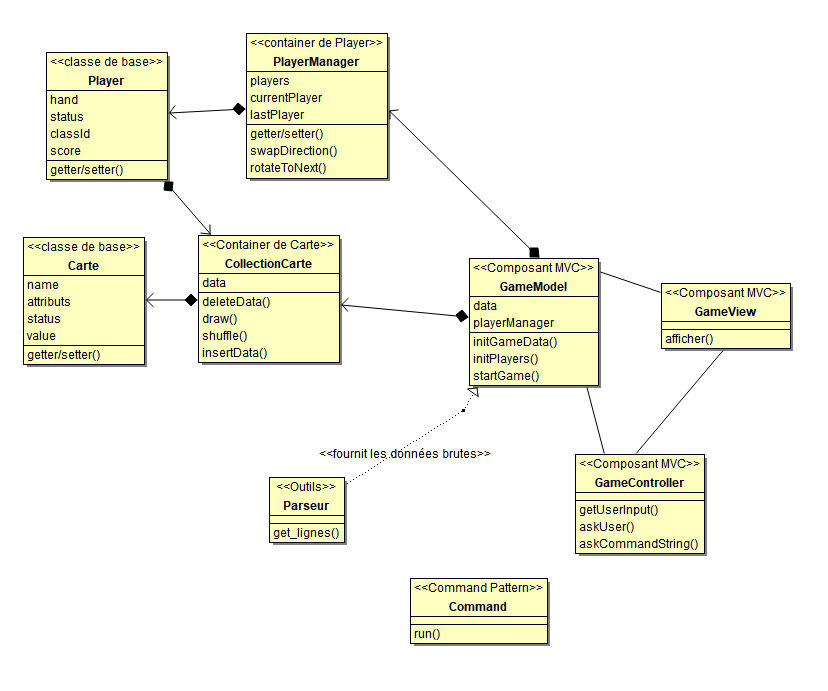
\includegraphics[width=\linewidth]{Diagramme.PNG}

\section{Présentation du jeu Uno realisé grâce à notre bibliothèque}
\subsection{Démarches de developpement}
Pour le jeux Uno j’ai décidé d’utiliser le cadre MVC que proposait notre bibliothèque, 
le début était plutôt simple car pour créer le deck de jeu, j’avais juste à écrire ma définition de pushDataFromStrLine \\

J’ai aussi créé une classe UnoCard, ce n’était pas si nécessaire mais cela apportait plus de visibilité à la structure de données,
plutôt que d’utiliser le vecteur de chaîne de charactere fourni par la classe Carte.\\
Une fois l’initiation faite, je n’avais plus qu’à écrire la boucle de jeu principale. J’ai du coup employé le Command Pattern dans ce but.\\
Le déroulement est très simple, afficher d’abord les informations utiles comme la main du joueur qui est en train de jouer.\\
Puis je propose au joueur de choisir une action qu’il souhaite exécuter.\\
Enfin je retrouve la bonne classe Command qui est associée à cette action.\\
Pour le Uno, l’utilisateur pouvait choisir entre "piocher" "jouer une carte" et "crier Uno".\\
Pour chaque action il existe alors une classe Command qui lui était associée.\\
Ainsi je peux me permettre de se concentrer sur l’action précise au lieu de tomber dans des boucles logiques de jeu interminable.\\
Cela apporte donc une meilleur visibilité, compréhension du code et une certaines modularités lors du développement.\\

A vrai dire nous n’avions pas besoin pour ces jeux d’une architecture MVC très sophistiqué, mais si on pense les choses un peu plus loin, cela est bénéfique. 
Imaginons qu’on décide un jour d’apporter une interface graphique à notre jeux, grâce à notre vue, le code du projet se modifiera que très peu. 
Nous avons besoin juste de changer la méthode affichage de notre vue.\\

\subsection{Diagramme de classe de UNO}

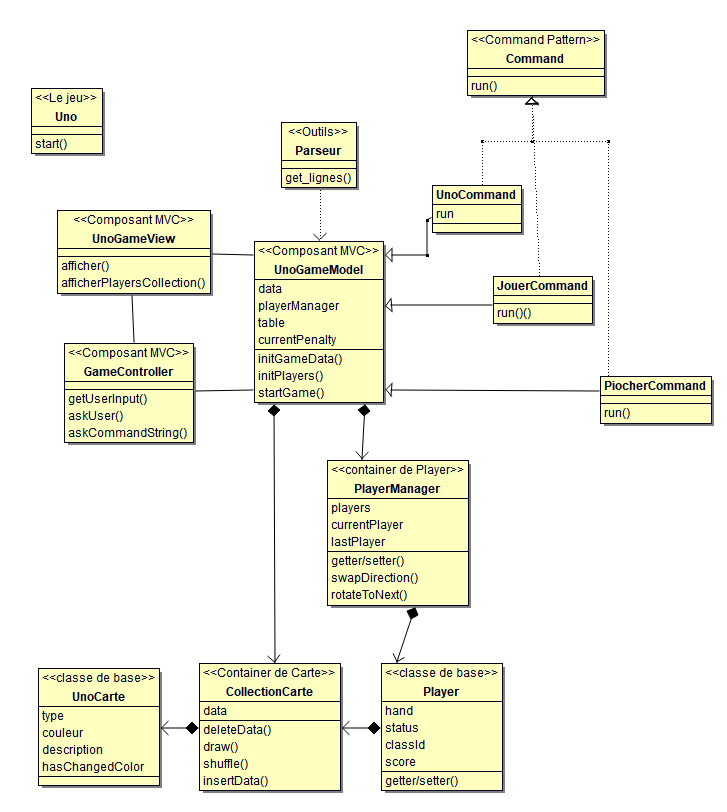
\includegraphics[width=\linewidth]{uno.PNG}
 
\end{document}
